\documentclass[a4paper]{oblivoir}

\title{쟤료공학개론 과제8}
\author{2018-12432, Electrical and Computer Engineering department, ParkJeonghyun}
\date{11/15/2023}

\newcommand{\be}{\begin{equation}}
\newcommand{\ee}{\end{equation}}

\usepackage{fapapersize}
\usepackage{amsmath}
\usepackage{MnSymbol}
\usepackage{wasysym}
\usepackage{graphicx}
\usepackage{caption}
\usepackage{subfig}
\usepackage{hyperref}
\usepackage{cite}
\usepackage{dtk-logos}
\usepackage{physics}
\usepackage{tikz}
\usetikzlibrary{decorations.markings, positioning}
\usepackage{dtk-logos}
\usepackage{fancyvrb}
\usepackage{array} 
\usepackage{chemformula}

\usefapapersize{ 210mm, 297mm, 15mm, 15mm, 15mm, 15mm}
\DeclareGraphicsExtensions{.pdf, .png, .jpg}

\renewcommand{\figurename}{Figure}

\begin{document}

\maketitle
\section{Problem 1}
\subsection{a}
\begin{align}
	\Delta G &= V\Delta G_{v} + S \gamma\\
	&= a^{3}\Delta G_{v} + 6a^{2}\gamma
\end{align}
미분하면
\begin{align}
	\frac{\Delta G}{da} &= 3a^{2}\Delta G_{v} + 12a\gamma
\end{align}
따라서
\begin{align}
	a^{*} &= - \frac{4\gamma}{\Delta G_{v}}
\end{align}
\begin{align}
	\Delta G^{*} &= \frac{32\gamma^{3}}{\Delta G_{v}^{2}}
\end{align}

\subsection{b}
구와 비교하면 
\begin{align}
	\Delta G^{*}(cube) &= \frac{32\gamma^{3}}{\Delta G_{v}^{2}} > \Delta G^{*}(sphere) =\frac{16\pi\gamma^{3}}{3\Delta G_{v}^{2}}
\end{align}
면적대비 부피가 육면체가 크기 때문에 육면체인 경우가 $\Delta G^{*}$가 크다. 


\section{Problem 2}
\subsection{a}
\begin{align}
	r^{*} &= -\frac{2\gamma_{SL} T_{E}}{\Delta H_{v}\Delta T}\\
	&= - \frac{2\times0.255\times1725}{-2.53\times10^{9}\times319}m\\
	&= 1.09nm
\end{align}

\begin{align}
	\Delta G^{*} &= \frac{16\pi\gamma^{3}_{SL}T_{E}^{2}}{3\Delta H_{v}^{2}\Delta T^{2}}\\
	&=\frac{16\times3.141592\times0.255^{3}\times1725^{2}}{3\times(2.53\times10^{9})^{2}\times319^{2}}\\
	&= 1.27\times 10^{-18}J
\end{align}

\subsection{b}
Nickel은 FCC이므로 격자당 4개의 원자가 존재한다. 따라서
\begin{align}
	N &= \frac{\frac{4}{3}\pi r^{*3}}{a^{3}}\times4\\
	&= \frac{\frac{4}{3}\pi 1.09^{*3}}{0.360^{3}}\times4\\
	&= 465
\end{align}

\section{Problem 3}
\begin{align}
	1 - y &= \exp(-kt^{n})\\
	\ln{1-y} &= -kt^{n}\\
	\ln\left(\ln{1/(1-y)}\right) &= \ln k + n\ln t\\
\end{align}
따라서
\begin{align}
	( \ln\ln1/0.8 - \ln\ln1/0.2 ) / \ln12.6/28.2&= n\\
	&=2.4525363\\
	k &= \ln(1/(1-0.2))/280^{2.4525363}\\
	&= 2.22\times10^{-7}
\end{align}
따라서
\begin{align}
	t_{95} &= (\ln(1/(1-0.95))/2.22\times10^{-7})^{1/2.4525363}\\
	&= 807.7 s
\end{align}

\section{Problem 4}
\subsection{a}
$760^{o}C$이상으로 가열하고 $10^{5}$초 이상 유지한다.

\subsection{b}
$760^{o}C$이상으로 가열하고 $35^{o}C/s$보다 약간 작게 상온으로 온도를 내린다.

\subsection{c}
$760^{o}C$이상으로 가열하고 $35^{o}C/s$보다 약간 작게 상온으로 온도를 내린다.

\subsection{d}
$760^{o}C$이상으로 가열하고 $140^{o}C/s$보다 빠르게 상온으로 온도를 내린다.

%\begin{figure}[htbp]
%	\begin{centering}
%	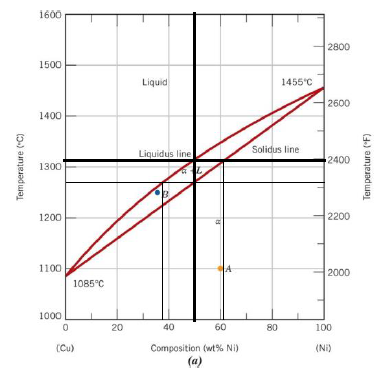
\includegraphics[width = 0.75\linewidth]{pro1.png}% Here is how to import EPS art
%	\caption{\label{fig:pro1} \ch{Ni-Co} Phase Diagram}
%	\end{centering}
%\end{figure}

\end{document}